\documentclass{beamer}
\usepackage[english]{babel}
\usepackage{calc}
\usepackage[absolute,overlay]{textpos}
\mode<presentation>{\usetheme{tud}}



\usepackage{tikz}
\usetikzlibrary{positioning,arrows}

\tikzset{
  block/.style={
    draw,
    rectangle,
    minimum height=1cm,
    minimum width=1cm,
    align=center
  },
  subblock/.style={
    draw,
    rectangle,
    minimum height=.75cm,
    minimum width=1.5cm,
    align=center
  },
  line/.style={->,>=latex},
  LED/.style={draw,circle,append after command={
        [shorten >=\pgflinewidth, shorten <=\pgflinewidth,]
        %(\tikzlastnode.north) edge (\tikzlastnode.south)
        %(\tikzlastnode.east) edge (\tikzlastnode.west)
        }
    },
  dot/.style={draw,circle,minimum size=2mm,inner sep=0pt,outer sep=0pt,fill=black},
  XOR/.style={draw,circle,append after command={
        [shorten >=\pgflinewidth, shorten <=\pgflinewidth,]
        (\tikzlastnode.north) edge (\tikzlastnode.south)
        (\tikzlastnode.east) edge (\tikzlastnode.west)
        }
    }
}

\usepackage{pifont}% http://ctan.org/pkg/pifont
\newcommand{\cmark}{\ding{51}}%
\newcommand{\xmark}{\ding{55}}%



\usepackage{epstopdf}




\title[Mid-term Presentation]{Leveraging VLC for energy }
\subtitle{disaggregation in Smart Buildings}
\institute[TU Delft]{Delft University of Technology}
\author{Johnny Verhoeff}
\date{\today}

% Insert frame before each subsection (requires 2 latex runs)
\AtBeginSubsection[] {
	\begin{frame}<beamer>\frametitle{\titleSubsec}
		\tableofcontents[currentsection,currentsubsection]  % Generation of the Table of Contents
	\end{frame}
}
% Define the title of each inserted pre-subsection frame
\newcommand*\titleSubsec{Next Subsection}
% Define the title of the "Table of Contents" frame
\newcommand*\titleTOC{Outline}

% define a symbol which can be removed if you don't need it
\newcommand{\field}[1]{\mathbb{#1}}
\newcommand{\Zset}{\field{Z}}

\begin{document} {
	% remove the next line if you don't want a background image
	\usebackgroundtemplate{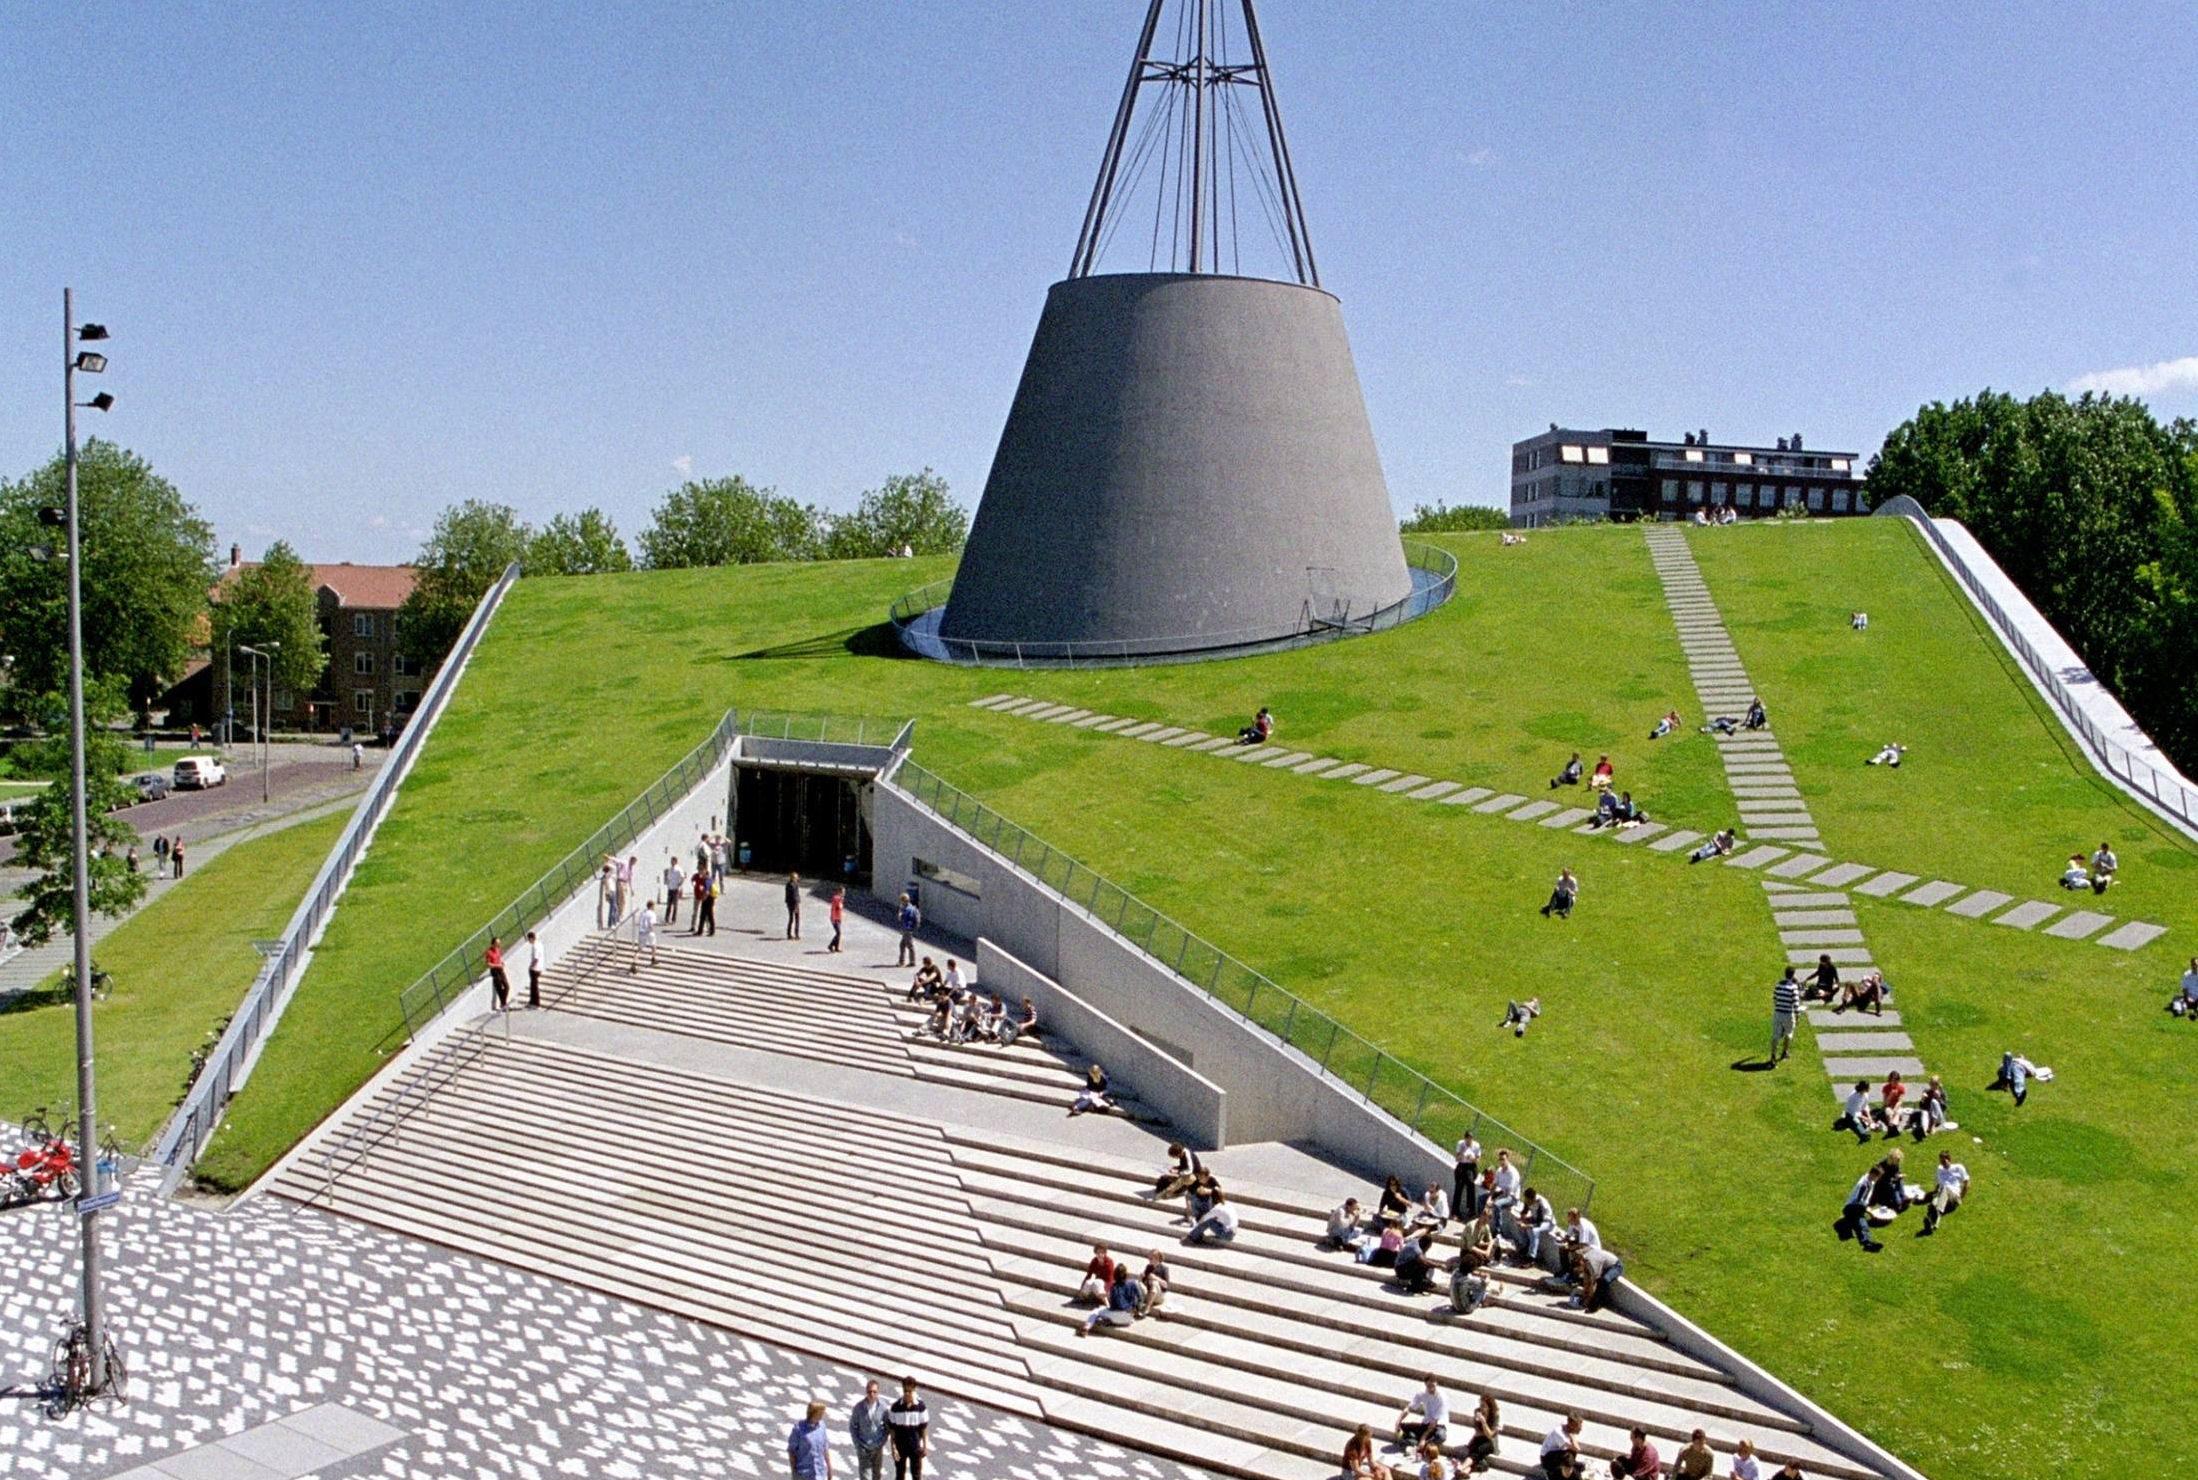
\includegraphics[width=\paperwidth,height=\paperheight]{images/background-titlepage.jpg}}%
	\setbeamertemplate{footline}{\usebeamertemplate*{minimal footline}}
	\frame{\titlepage}
}

\beamertemplatenavigationsymbolsempty
%\setbeamertemplate{navigation symbols}{}

\setbeamertemplate{caption}{\raggedright\insertcaption\par}

%{\setbeamertemplate{footline}{\usebeamertemplate*{minimal footline}}
%\begin{frame}\frametitle{\titleTOC}
%	\tableofcontents
%\end{frame}
%}

%\section{First Section}
%\subsection{Section 1 - Subsection 1}


	%intro
	\begin{frame}\frametitle{Energy Disaggregation}

		Energy consumption is a most pressing issue.

		\begin{itemize}

			\item To reduce it, understanding the usage of that energy is needed.

			\item Smart-meter can disaggregate the energy usage in a household.

			\item This is done by recognizing the unique signatures of appliances.

		\end{itemize}

		\begin{figure}[t]
			\centering
			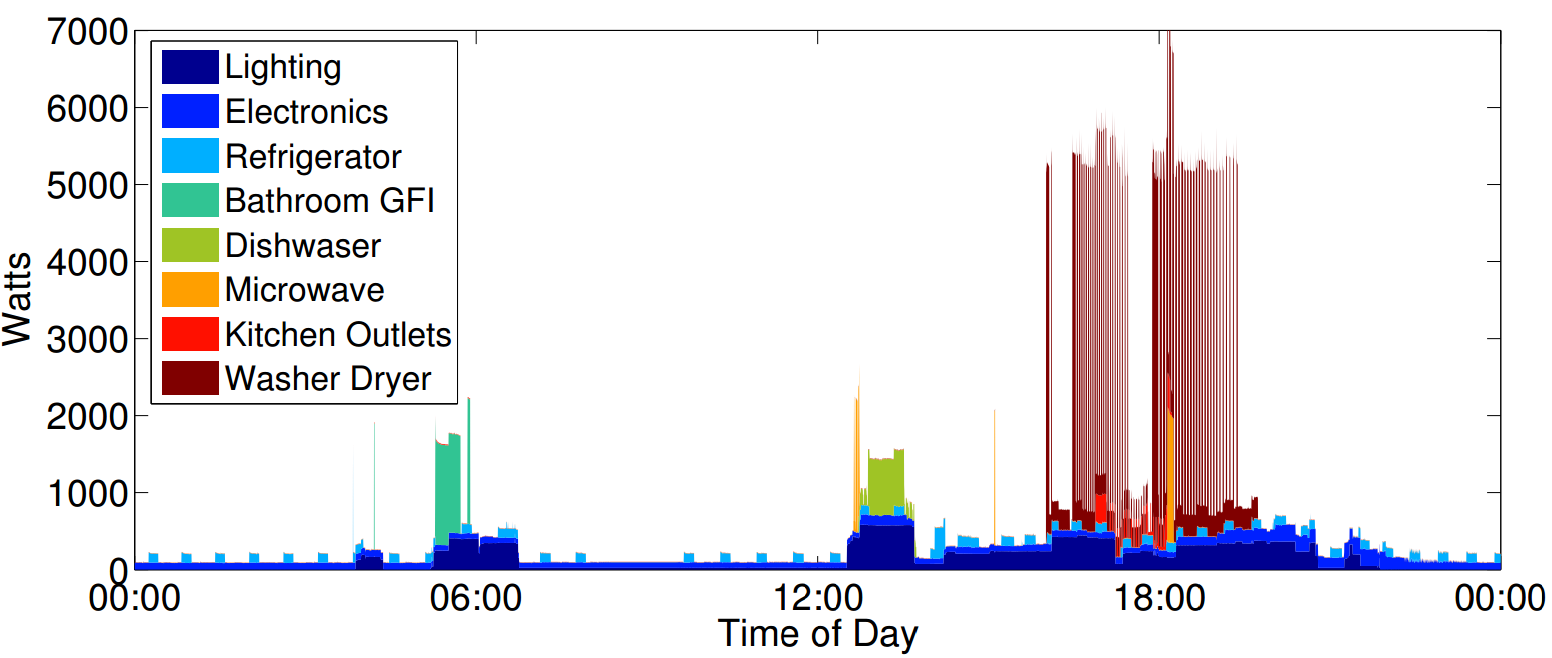
\includegraphics[width=0.7\textwidth]{../chapters/introduction-chapters/energy-consumption-house.png}
		\end{figure}

		% For example here we can see the aggregated energy from a household during a day.
		% With the different colors it is indicated what appliance is being used at what time.
		% In the blue we can see 'lighting' as a constant consumer but it can not disaggregate which individual lights are on.

	\end{frame}






	\begin{frame}\frametitle{Lighting Energy}

		Individual lights cannot be disaggregated (yet).

		\begin{itemize}

			\item The reason: Lighting does not have a unique signature. %Which HVAC for example does have.

			\item Instead there are many lights with the same signature.

			\item Still important to be able to disaggregate individual lights: Lighting consumes 19 \% of the power in an average household.

		\end{itemize}


	\end{frame}





	\begin{frame}\frametitle{VLC}

		VLC is a communication method which uses visible light to transmit data.

		\begin{itemize}

			\item This data can be unique IDs for LED beacons used for indoor localization.

			\item This data will also propagate through the current draw.

			\item Can we construct these IDs in such a way that the aggregated current can be disaggregated by a smart-meter ?

		\end{itemize}

	\end{frame}



	\begin{frame}\frametitle{Overview}

		%Smart-meter will measure aggregated current draw of all LEDs.

		\begin{figure}
			\centering
			\resizebox {0.8\textwidth} {!} {
				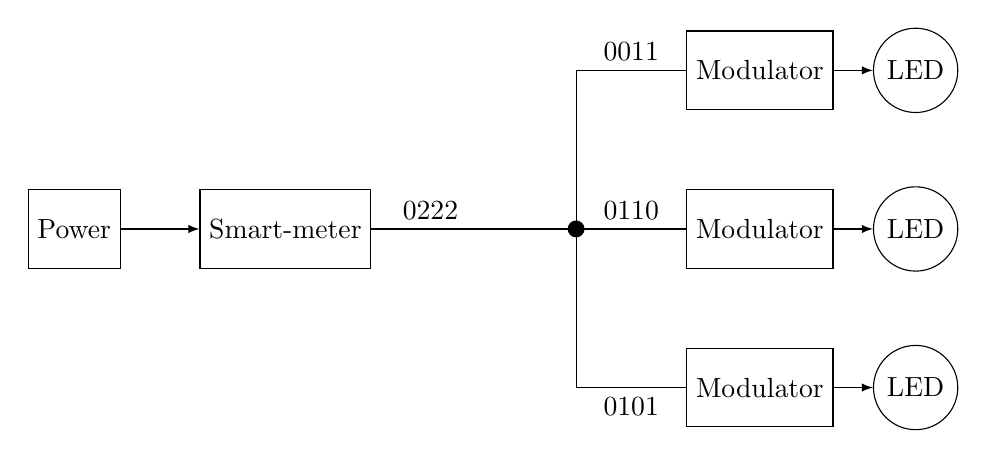
\begin{tikzpicture}

					\node[block] (smart_meter) {Smart-meter};	

					\node[block, left = 1cm of smart_meter] (power) {Power};	
					\draw[line] (power.east) -- (smart_meter.west) node [midway, right] {};		

					% second mod.
					\node[block, right = 4cm of smart_meter] (second_modulator) {Modulator};
					\node[LED, right = 0.5cm of second_modulator] (second_led) {LED};
					\draw[line] (second_modulator.east) -- (second_led.west) node [midway, right] {};

					% first mod.
					\node[block, above = 1cm of second_modulator] (first_modulator) {Modulator};
					\node[LED, right = 0.5cm of first_modulator] (first_led) {LED};
					\draw[line] (first_modulator.east) -- (first_led.west) node [midway, right] {};

					% third mod.
					\node[block, below = 1cm of second_modulator] (third_modulator) {Modulator};
					\node[LED, right = 0.5cm of third_modulator] (third_led) {LED};
					\draw[line] (third_modulator.east) -- (third_led.west) node [midway, right] {};

					\node[dot, right = 2.5cm of smart_meter] (CP) {};

					\draw (smart_meter.east) -- (CP) node [pos=0.3, above] {0222};

					\draw (CP) |- (first_modulator.west) node  [pos=0.75, above] {0011};
					\draw (CP) |- (second_modulator.west) node [pos=0.75, above] {0110};
					\draw (CP) |- (third_modulator.west) node  [pos=0.75, below] {0101};

				\end{tikzpicture}
			}
		\end{figure}

		\begin{itemize}

			\item What type of codes can be used as IDs for the LEDs ?

			\item Which hardware is required to modulate and disaggregate these codes ? 

			\item Evaluate the solutions.

		\end{itemize}

	\end{frame}





	




	\begin{frame}\frametitle{Recognizing the IDs}
		
		Correlation: Measuring the similarity between a code and a received signal:

		\begin{equation*}
			R(\tau)_{xy} = \displaystyle\sum_{i = 0} ^ {L - 1} x(i) \times y(i + \tau) {\text{  with $\tau = 0, 1, 2, \dotsc, L$}}
		\end{equation*}

		\begin{itemize}

			\item Auto-correlation: When the signal is present, it should yield a high value.

			\item Cross-correlation: When the signal is NOT present, it should yield a low value.

		\end{itemize}
	\end{frame}



	\begin{frame}\frametitle{Requirements for Codes}
		
		\begin{itemize}

			\item Correlation:
			\begin{itemize}

				\item Auto-correlation should be high.

				\item Cross-correlation should be low.

			\end{itemize}

			\item The ability to work in synchronous and asynchronous scenarios.

			\item The codes should be not too long.

			\item The number of codes should scale well with the length of the code. 

		\end{itemize}
		
	\end{frame}



	\begin{frame}\frametitle{Orthogonal Codes}
		\begin{itemize}

			\item Creation via Hadamard matrix: 
			\begin{equation*}
				H_{2n} = 
				\begin{bmatrix} 
					H_n & H_n \\ 
					H_n & -H_n 
				\end{bmatrix}
			\end{equation*}

			\item Auto-correlation is high, only in synchronous scenario.

			\item Cross-correlation is low and math. bounded, only in synchronous scenario.

			\item $C \propto L$


		\end{itemize}
		

	\end{frame}


	\begin{frame}\frametitle{PN Codes}
		\begin{itemize}
			\item Creation of a PN code via LFSR:
		
				\begin{figure}[t]
					\centering
					\resizebox {0.8\textwidth} {!} {
						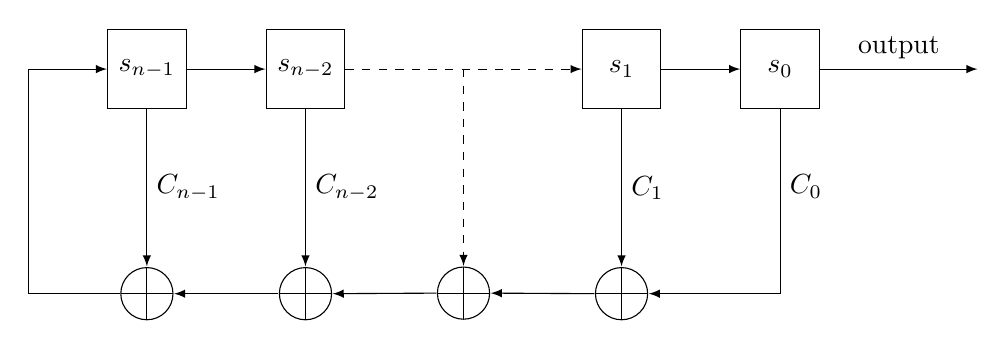
\begin{tikzpicture}


							\node[block                  ] (last_register) {$s_{n-1}$};
							\node[block, right = 1cm of last_register] (second_last_register) {$s_{n-2}$};
							\draw[line] (last_register.east) -- (second_last_register.west) ;

							\node[block, right = 3cm of second_last_register] (second_register) {$s_{1}$};
							\node[block, right = 1cm of second_register] (mid_register) {$s_{0}$};
							\draw[line] (second_register.east) -- (mid_register.west) ;

							\draw[dashed, line] (second_last_register.east) -- (second_register.west) ;

							\node[coordinate, right = 2cm of mid_register] (output_point) {};
							\draw[line] (mid_register.east) -- (output_point.west) node [midway, above] {output};

							\node[XOR, scale=2, below = 2cm of second_register] (first_xor) {};
							\draw[line] (second_register.south) -- (first_xor.north) node [midway, right] {$C_1$};
							\draw[line] (mid_register.south) |- (first_xor.east) node [pos=0.21, right] {$C_0$};

							\node[coordinate, right = 1.5cm of second_last_register] (h) {};
							\node[XOR, scale=2, below = 2.5cm of h] (mid_xor) {};
							\draw[line] (first_xor.west) -- (mid_xor.east) ;
							\draw[dashed, line] (h.south) -- (mid_xor.north) ;

							\node[XOR, scale=2, below = 2cm of second_last_register] (second_last_xor) {};
							\node[XOR, scale=2, below = 2cm of last_register] (last_xor) {};

							\draw[line] (second_last_register.south) -- (second_last_xor.north) node [midway, right] {$C_{n-2}$};
							\draw[line] (mid_xor.west) -- (second_last_xor.east) ;
							
							\draw[line] (second_last_xor.west) -- (last_xor.east) ;
							\draw[line] (last_register.south) -- (last_xor.north) node [midway, right] {$C_{n-1}$};

							\node[coordinate, left = 1cm of last_register] (return_point) {};
							
							\draw[line] (last_xor.west) -| (return_point) -- (last_register.west) ;

						\end{tikzpicture}
					}
				\end{figure}

			\item Auto-correlation is high, in synchronous and asynchronous scenarios.

			\item Cross-correlation: Exhaustive analysis is required.

			\item $C = \frac{1}{n} \prod \{ P_{i} ^ {(\alpha_i - 1)} \times (P_i - 1) \}$ $\rightarrow$ $C \not\propto L$


		\end{itemize}
		

	\end{frame}



	\begin{frame}\frametitle{Gold Codes}
		\begin{itemize}
			\item Creation of a Gold code via two separate LFSRs.

			\item Auto-correlation is high, in synchronous and asynchronous scenarios.

			\item Cross-correlation is low and math. bounded in synchronous and asynchronous scenarios.

			\item $C \propto L$


		\end{itemize}
		

	\end{frame}










	\begin{frame}\frametitle{Comparison of Codes}
		

		\begin{table}
			\centering
			\resizebox {\textwidth} {!} {
				\begin{tabular}{ | l | l | l | l | }

					\hline
																	& Orthogonal 	& PN 		& Gold 		\\ \hline
					Synchronous	Transmission						& \cmark		& \cmark	& \cmark	\\ \hline
					A-synchronous Transmission						& \xmark		& \cmark	& \cmark	\\ \hline
					Math. bounded CC (synch.)						& \cmark		& \xmark	& \cmark	\\ \hline
					Math. bounded CC (asynch.)						& \xmark		& \xmark	& \cmark	\\ \hline
					Scalability ($C \propto L$)						& \cmark		& \xmark	& \cmark	\\ \hline		


				\end{tabular}
			}

		\end{table}
	\end{frame}





	\begin{frame}\frametitle{Mapping Problem}

		\begin{itemize}

			\item VLC is most commonly used with OOK symbols: 0 (off) and 1 (on).

			\item Codes explained use symbols: $+1$ and $-1$: $\rightarrow$ balanced around $0$.

			\item Mapping must take place between these two sets of symbols: $b = \frac{1 - r}{2}$.

			\item Use this mapping to figure out how to calculate the correlations.

		\end{itemize}
	\end{frame}



	\begin{frame}\frametitle{Interference Solution}

		Cross-correlation is not negligible.

		\begin{itemize}

			\item The maximum number of concurrent transmitters $m$ can be calculated, such that no interference will take place : $L = f(m)$.

			\item Other way: probabilistic approach.

		\end{itemize}


	\end{frame}


	\begin{frame}\frametitle{Probabilistic Approach}

		\begin{itemize}

			\item Accuracy: determines the accuracy in identifying which LEDs are on and off. And outputs a probability $p$ for which the LEDs will modulate.

			\item Approximate the time it will take to successfully identify all LEDs: $t = f(L,\ f,\ p)$

		\end{itemize}
		
	\end{frame}


















	\begin{frame}\frametitle{Hardware Components}

		Components that will be investigated: 

		\begin{itemize}

			\item LED modulator

			\item Current sampler (smart-meter)

		\end{itemize}
		
	\end{frame}



	\begin{frame}\frametitle{Understanding AC Voltage}

		\begin{figure}
			\centering
			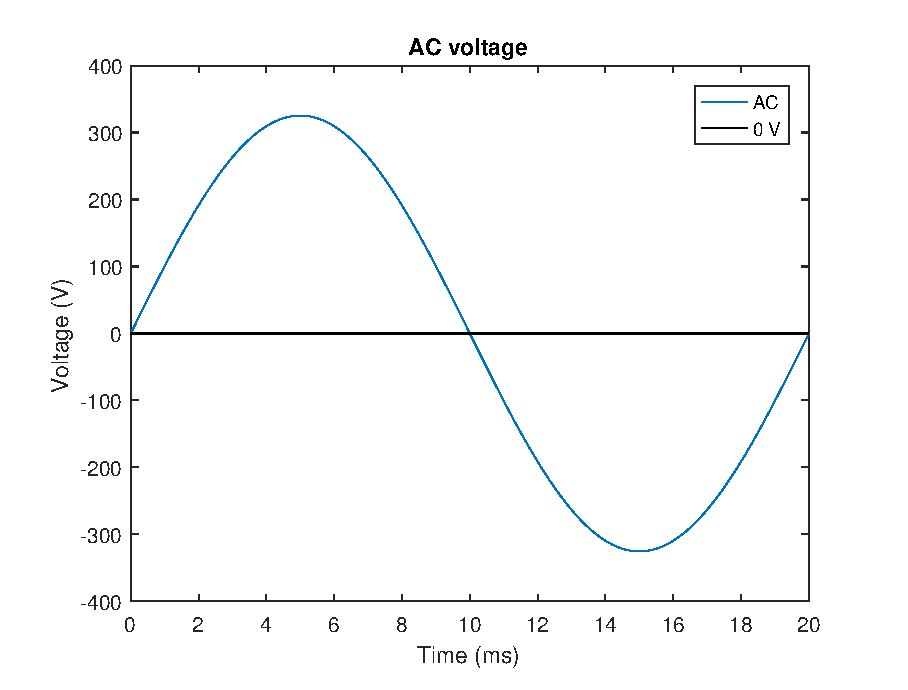
\includegraphics[width=0.6\textwidth]{ac-wave.eps}
		\end{figure}

		AC characteristics:

		\begin{itemize}

			\item Supplied voltage is not constant.

			\item Supplied voltage will be both positive and negative.

		\end{itemize}
		
	\end{frame}






	\begin{frame}\frametitle{Existing Modulator Hardware}

		\begin{figure}
			\resizebox {0.8\textwidth} {!} {
			  \centering
			  \begin{minipage}[b]{0.48\textwidth}
			    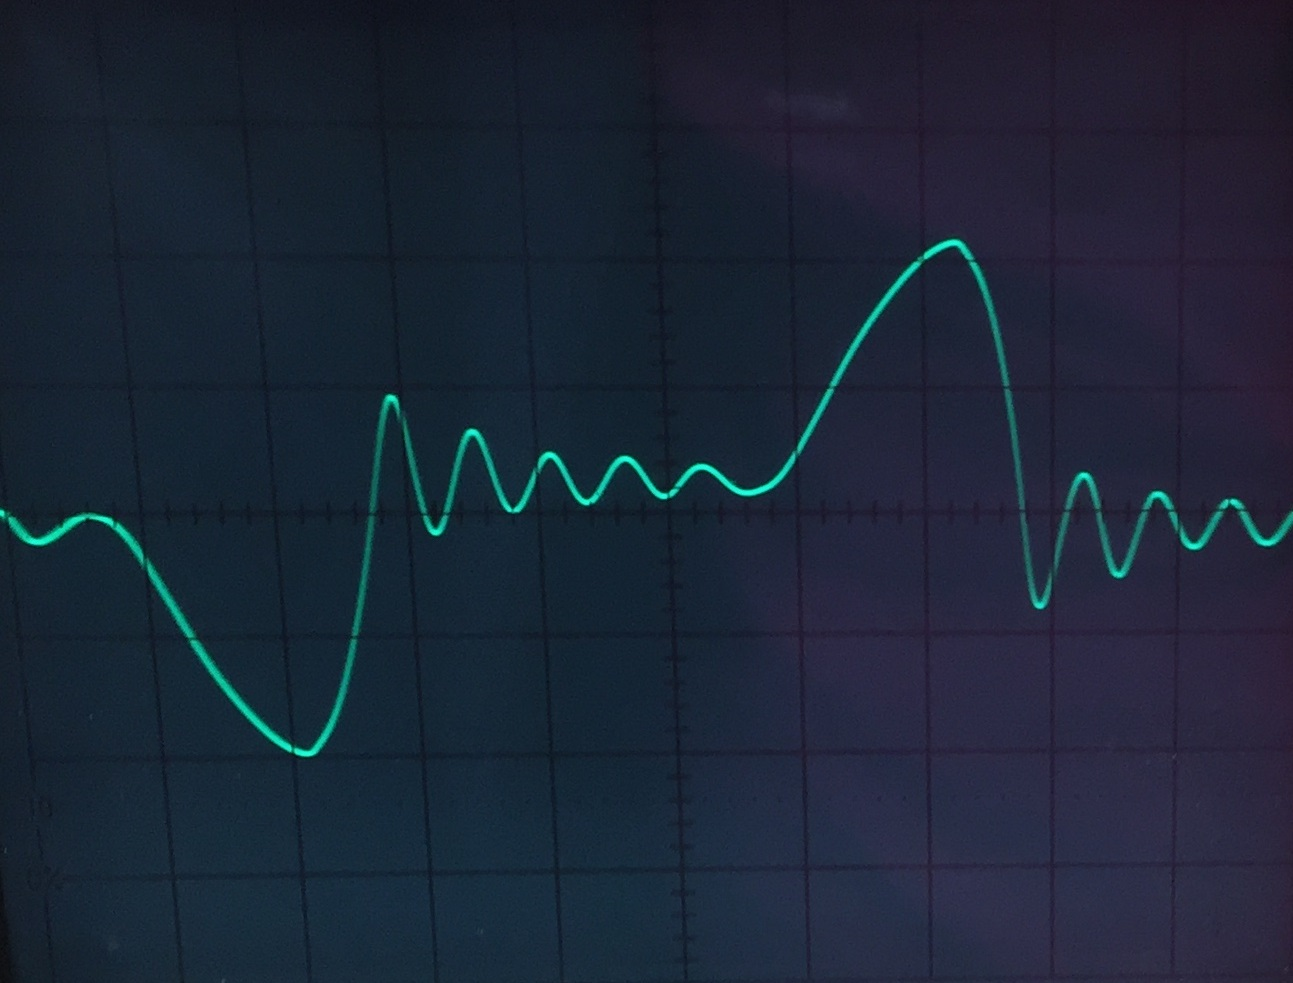
\includegraphics[width=\textwidth]{../chapters/hardware-chapters/smps-current-primary-with-load-cropped.jpg}
			    \caption{Switching Mode Power Supply}
			  \end{minipage}
			  \hfill
			  \begin{minipage}[b]{0.4\textwidth}
			    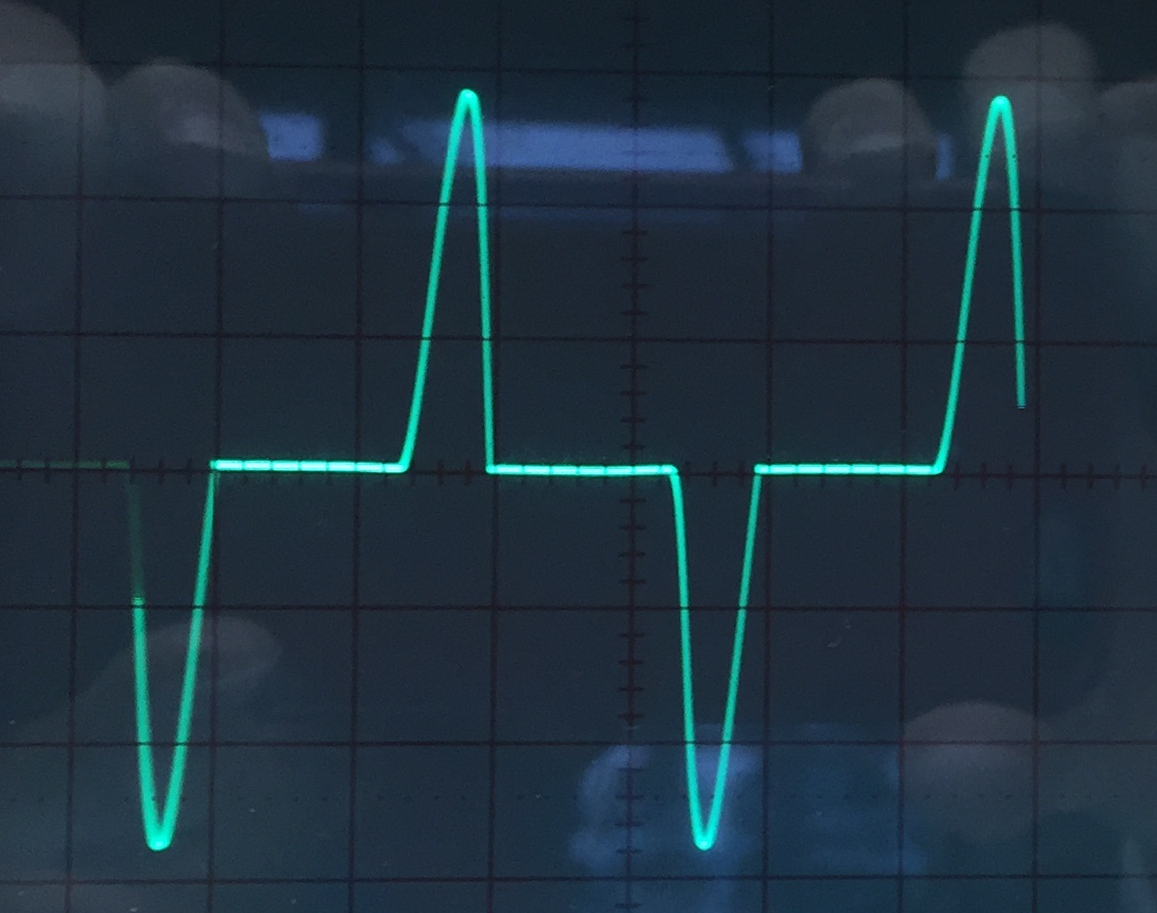
\includegraphics[width=\textwidth]{../chapters/hardware-chapters/commercial-230v-ac-led-on-cropped.png}
			    \caption{Commercial AC LED}
			  \end{minipage}
		  }
		\end{figure}

		These solutions will not yield nice aggregated signals.
		
	\end{frame}




	\begin{frame}\frametitle{Detecting When to Modulate}

		\begin{itemize}

			\item AC Voltage is zero crossing.

			\item LEDs require some voltage before the current starts flowing.

		\end{itemize}
		

		\begin{figure}
			\centering
			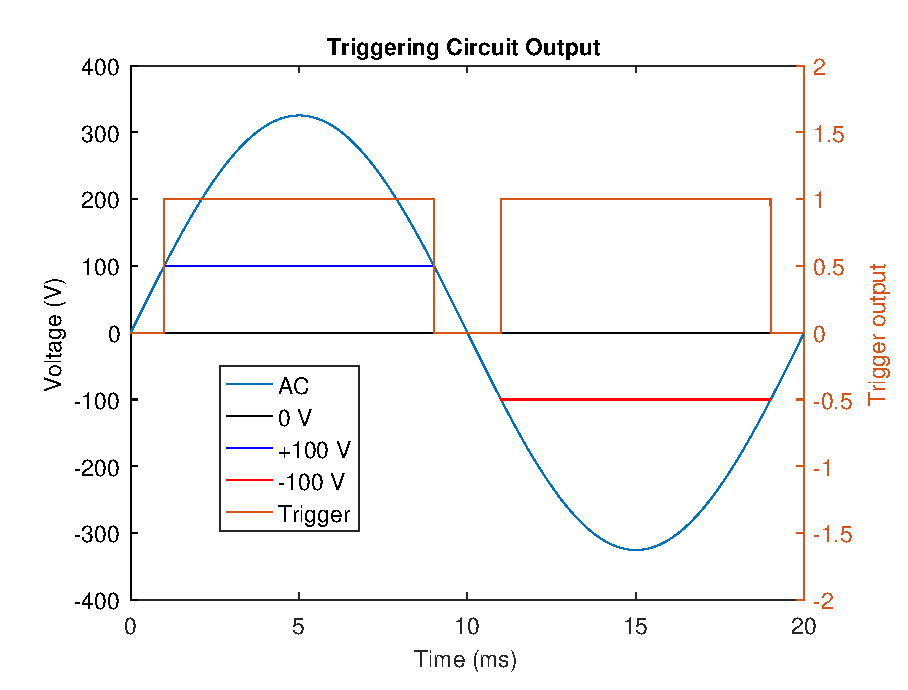
\includegraphics[width=0.7\textwidth]{ac-wave-triggering.eps}
		\end{figure}
		
		
	\end{frame}



	\begin{frame}\frametitle{Constant Current Draw}


		\begin{itemize}

			\item AC Voltage is not constant.

			\item For disaggregation a flat constant current is desired.

		\end{itemize}

		\begin{figure}
			\centering
			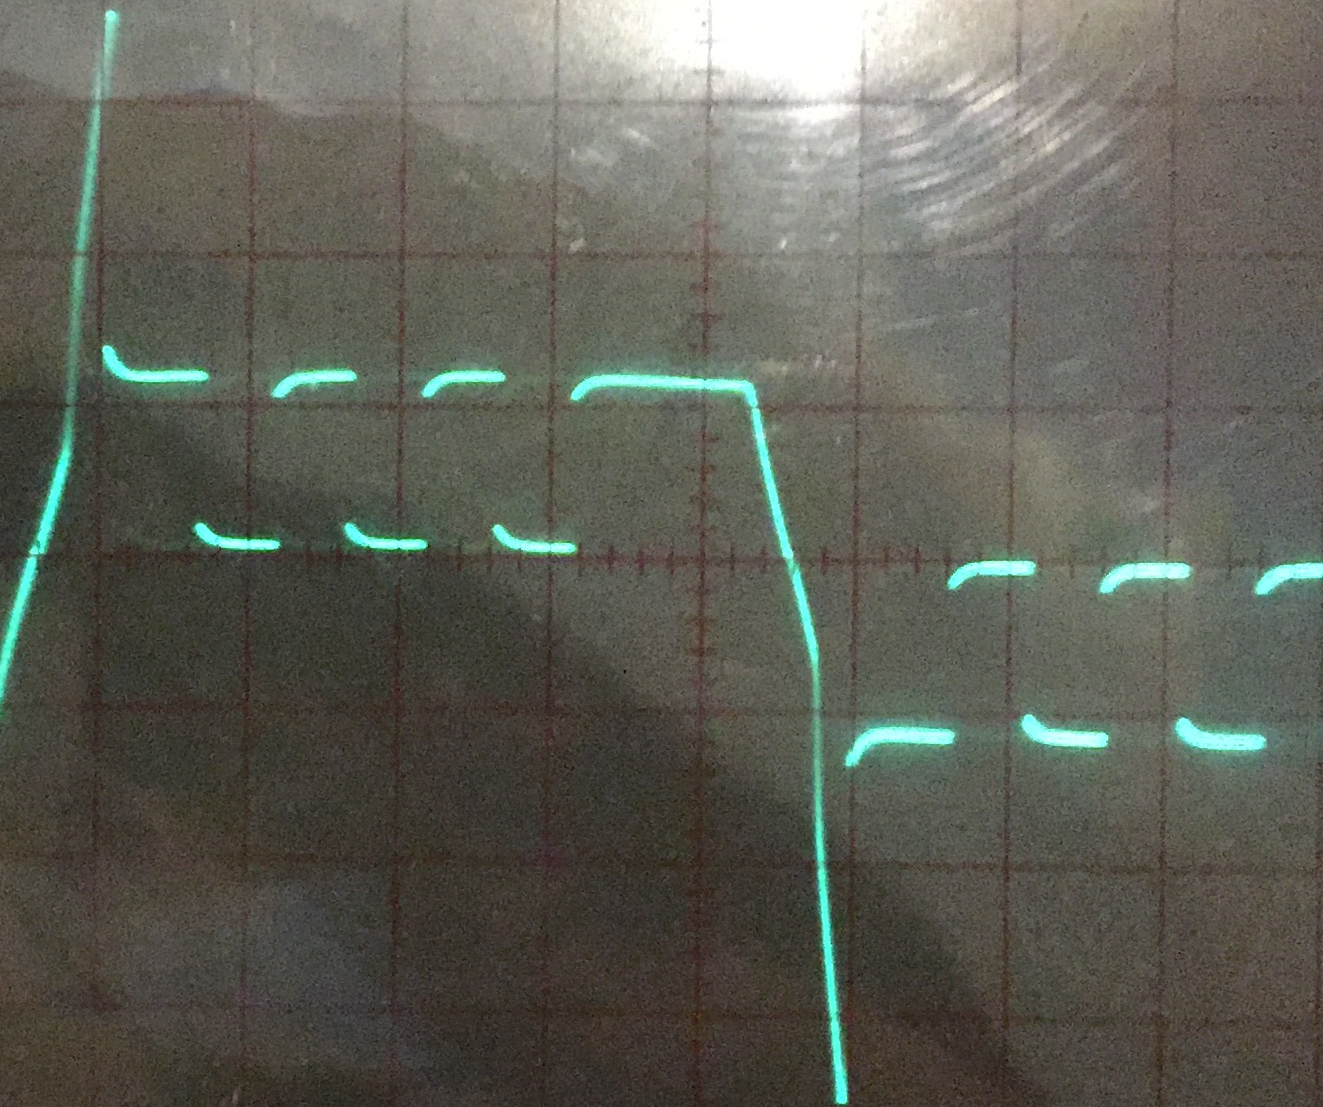
\includegraphics[width=0.6\textwidth]{../chapters/hardware-chapters/current-source-measurement-cropped.png}
			\caption{Constant current source}
		\end{figure}


	\end{frame}



	\begin{frame}\frametitle{Smart meter}

		AC Current sampler options:

		\begin{columns}
			\begin{column}{0.48\textwidth}

				\begin{itemize}
					\item Hall effect sensor:

					\begin{itemize}
						\item Sensitivity: 185 mV / A
						\item Noise: 21 mV
						\item Output: 15 W LED yields 12 mV 
						\item Noise $>$ output: not a viable option.
					\end{itemize}

					\item Burden resistor:

					\begin{itemize}
						\item Sensitivity: 2800 mV / A
						\item No noise 
						\item Output: 15 W LED yields 183 mV 
						\item Positive and negative voltage output %because of AC, so add a constant voltage to it and feed to an ADC
					\end{itemize}


				\end{itemize}
			\end{column}
			\begin{column}{0.48\textwidth}

				\begin{figure}
					\centering
					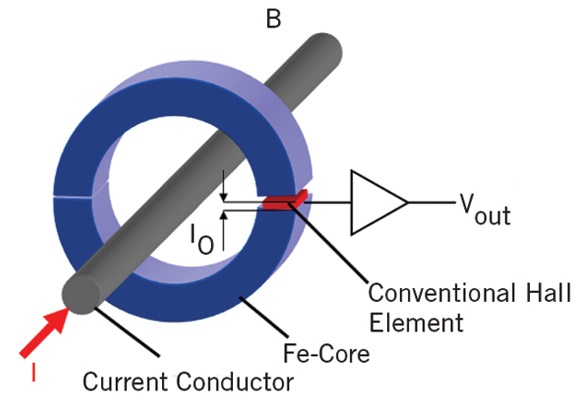
\includegraphics[width=0.8\textwidth]{hall-effect-sensing}
				\end{figure}

			\end{column}
		\end{columns}


		

		
		
	\end{frame}




	\begin{frame}\frametitle{Recap}
		
		Goals: 

		\begin{itemize}

			\item Codes for LEDs that can be identified when used with other codes.

			\item Detection and identification must be done in a timely manner.

		\end{itemize}
	\end{frame}





	\begin{frame}\frametitle{Setup for Hardware Evaluation}
		

		\begin{itemize}

			\item The setup consists of 3 individual controllable commercial LEDs + current sampler.

			\item All LEDs are transmitting continuously with a code that support at least 3 concurrent transmitters.

			\item The goal is to identify a LED as being on without seeing interference from the other LEDs.

			\item Another goal is to check if another code which is not used for any LED, can be identified. This should NOT be the case, because this LED is not present.


		\end{itemize}
	\end{frame}




	\begin{frame}\frametitle{Raw ADC Data}

		\begin{figure}
			\centering
			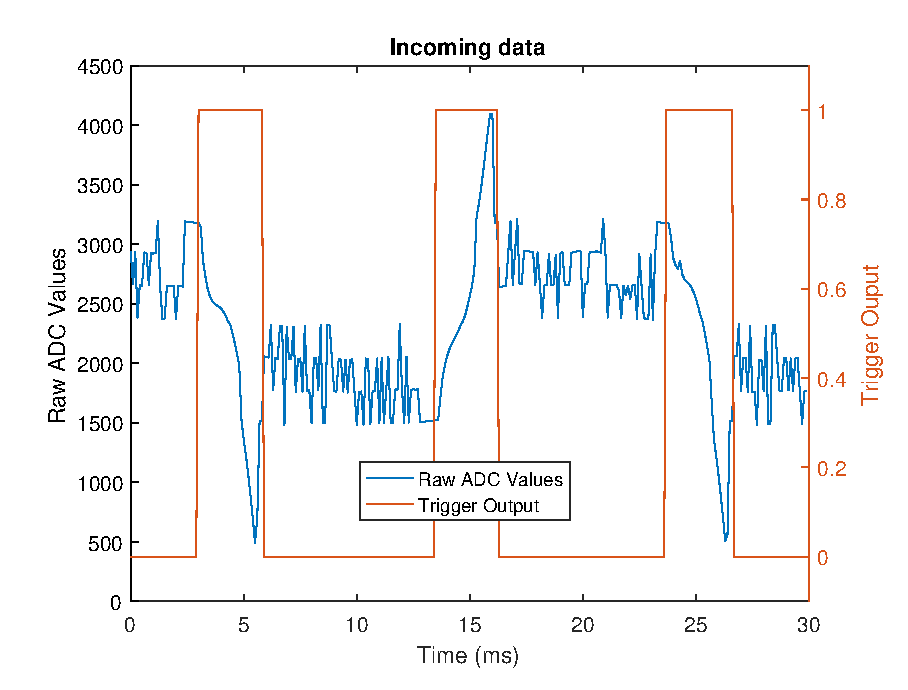
\includegraphics[width=0.8\textwidth]{ac-raw-data.eps}
		\end{figure}

	\end{frame}

	\begin{frame}\frametitle{Processed ADC Data}

		\begin{figure}
			\centering
			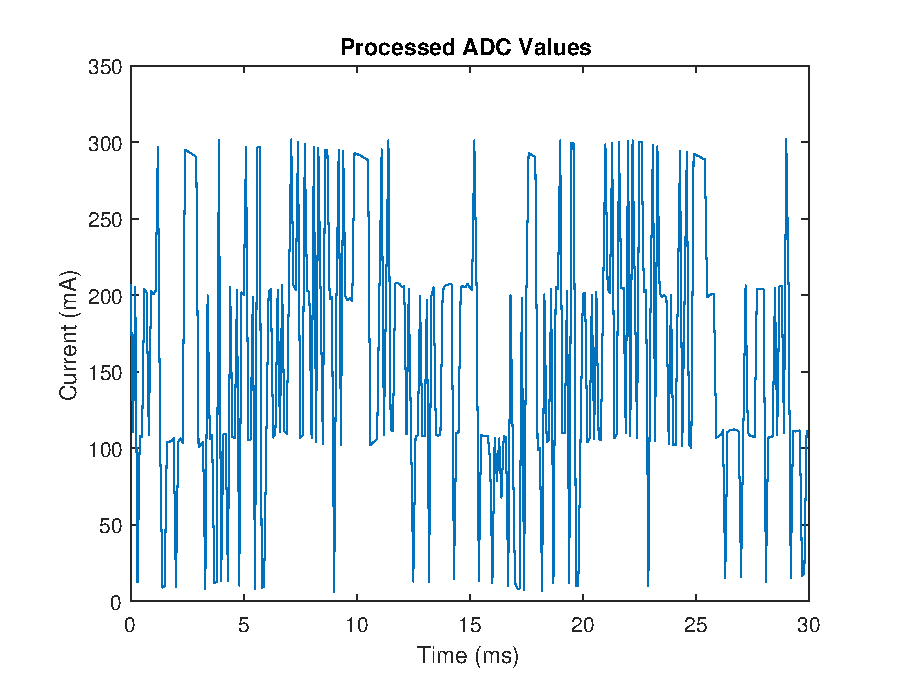
\includegraphics[width=0.8\textwidth]{ac-processed-data.eps}
		\end{figure}

	\end{frame}

	\begin{frame}\frametitle{Identifying LEDs}

		\begin{figure}
			\centering
			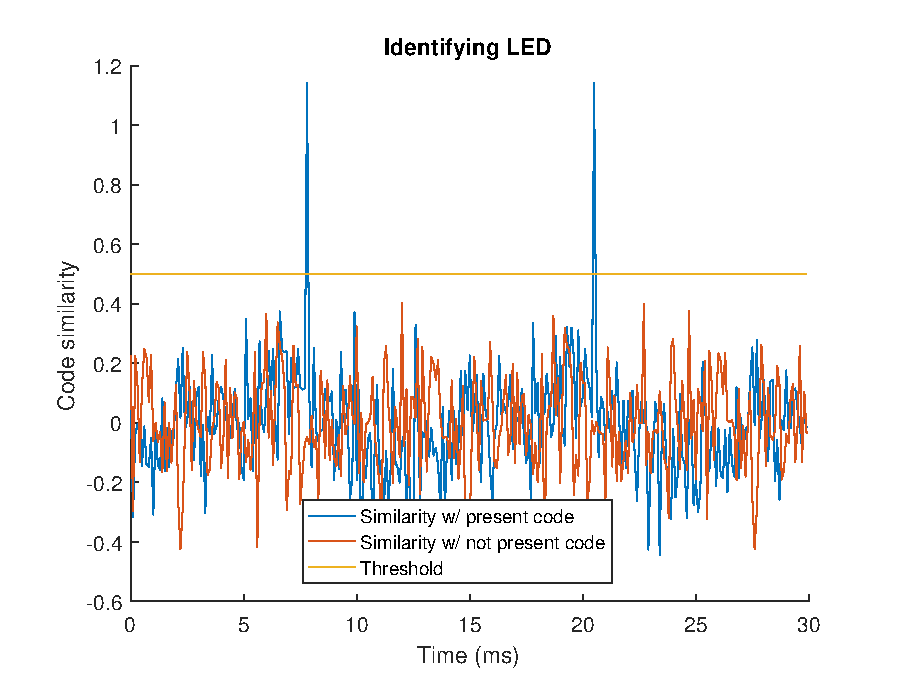
\includegraphics[width=0.8\textwidth]{correlation-results.eps}
		\end{figure}

	\end{frame}











	\begin{frame}\frametitle{Simulation}
		
		To be able to test larger systems, simulations are used.

		Assuming 129 individual LEDs which follow the probabilistic scheme.

	\end{frame}



	\begin{frame}\frametitle{Simulation}
		
		\begin{figure}[t]
			\centering
			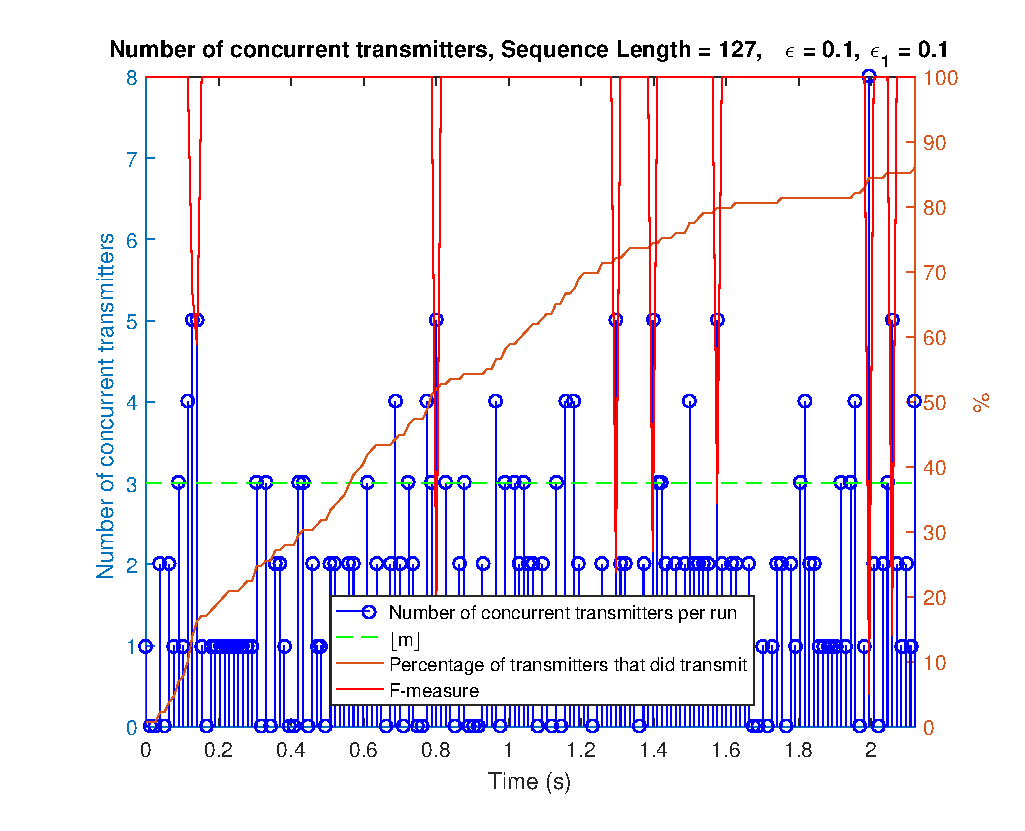
\includegraphics[width=0.8\textwidth]{simulation-1.eps}
		\end{figure}

		% With this probabilistic scheme, the settings are a bit high, which will result in fast times but low completeness and decoding errors.
		% Every time the number of concurrent transmitters goes above the m line, interference MAY happen, below the line everything will be fine, this is proven.
		% WHen the interference happens fp and fn may occur and we see the f-measure drop.
		% for 129 transmitters it takes 2.1 seconds to let 85 % of the transmitters transmit.

	\end{frame}

	\begin{frame}\frametitle{Simulation (2)}
		
		\begin{figure}[t]=
			\centering
			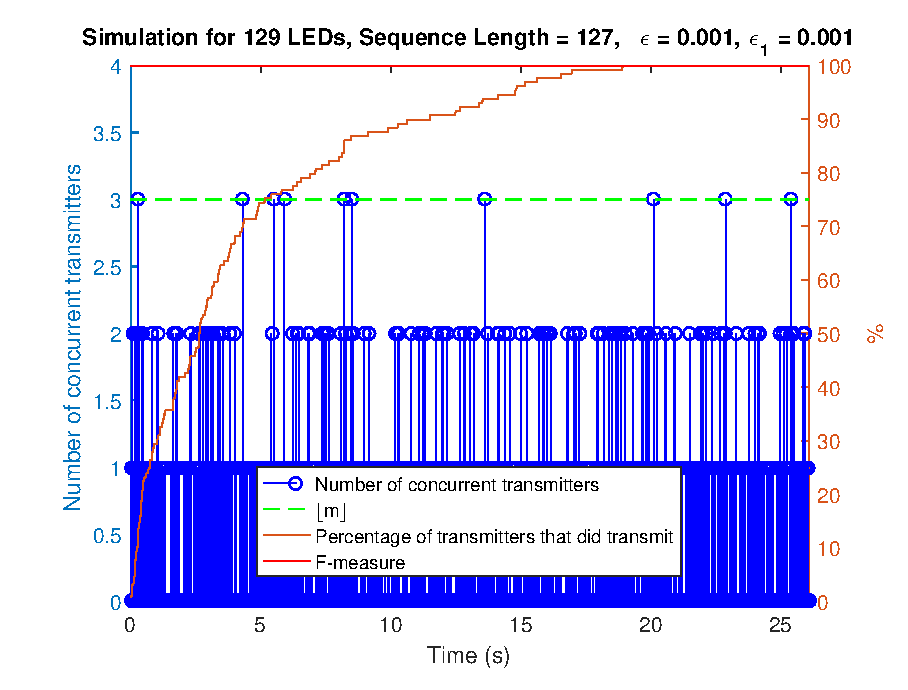
\includegraphics[width=0.8\textwidth]{simulation-2.eps}
		\end{figure}

		% In this simulation we still have the same number of transmitters, 129, but we require more precision and completeness.
		% We see that it takes more time to complete: around 26 seconds but 99 % of the transmitters have actually transmitted 
		% and only one time was there too much interference.


	\end{frame}











\end{document}
